
%(BEGIN_QUESTION)
% Copyright 2006, Tony R. Kuphaldt, released under the Creative Commons Attribution License (v 1.0)
% This means you may do almost anything with this work of mine, so long as you give me proper credit

Examine this flow control system, where a valve controls the flow rate of liquid between two vessels:

$$\includegraphics[width=15.5cm]{i01458x01.eps}$$

Since each vessel has its liquid level controlled by an overflow pipe, the head pressure at the bottom of each will be constant.  This means that the differential pressure across the valve will be constant as well.

\vskip 10pt

Suppose now that the higher vessel has its overflow pipe moved to a lower location, thus reducing the controlled level in that vessel, and consequently the head pressure generated at the bottom:

$$\includegraphics[width=15.5cm]{i01458x02.eps}$$
 
This change in head pressure, of course, reduces the amount of differential pressure across the valve.  How will this affect the process gain, as it relates to flow control?  In other words, will the flow rate become more or less sensitive to changes in valve position as a result of decreasing the pressure drop across the valve?

\vskip 10pt

What will happen to the process gain if we then replace the control valve with one having a larger $C_v$ value (a larger opening for fluid flow when fully open)?

\vskip 10pt

Finally, what will happen to the process gain if we re-calibrated the flow transmitter for a smaller span (for example, from 0-120 GPM to 0-75 GPM)?

\underbar{file i01458}
%(END_QUESTION)





%(BEGIN_ANSWER)

Reducing the differential pressure drop across the valve will result in less flow when the valve is fully open.  Of course, the flow rate will still be zero when the valve is fully closed.  This means that the controllable flow {\it range} has been decreased as a result of decreased pressure drop across the valve.

With less of a controllable flow range, the flow will not change as much as it did before given the same change in valve position.  That is to say, the process variable in this control system will be less sensitive to changes in valve position than before.  In other words, we are faced with a {\it decreased} process gain.

\vskip 10pt

Given a larger valve, the process gain will {\it increase}, because greater changes in flow rate will result from the same changes in valve position with a valve of greater size.

Technically speaking, the gain of the valve (ratio of valve coefficient, or C$_{v}$, versus position change) is a separate variable from the gain of the process itself (ratio of flow rate versus valve coefficient), and this is separate from the gain of the sensor (ratio of transmitter output percentage versus flow rate).  However, here I use the term ``process gain'' to refer to the sensitivity of the whole control system, except the controller (the process vessels and piping, control valve, and flow transmitter).

\vskip 10pt

Given a flow transmitter with a smaller range, the process gain will {\it increase}, because the same changes in valve position will now result in greater {\it percentage} changes in the transmitter output.

%(END_ANSWER)





%(BEGIN_NOTES)


%INDEX% Control, proportional: process gain

%(END_NOTES)


